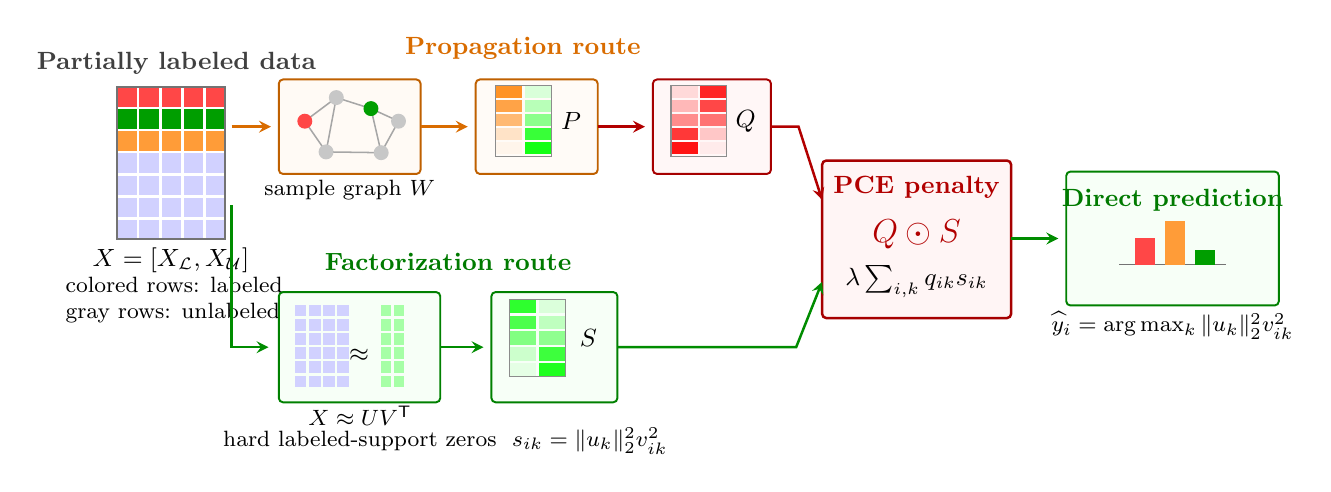
\begin{tikzpicture}[
  font=\small,
  >=stealth,
  flow/.style={->,line width=0.9pt},
  orangeflow/.style={flow,draw=orange!85!black},
  greenflow/.style={flow,draw=green!55!black},
  redflow/.style={flow,draw=red!70!black},
  module/.style={rounded corners=1.5pt,line width=0.7pt,fill=white},
  labelbox/.style={align=center,font=\small\bfseries}
]
% Input matrix with labeled and unlabeled samples.
\node[labelbox,text=black!75] at (0.85,4.85) {Partially labeled data};
\foreach \r in {0,...,6}{
  \foreach \c in {0,...,4}{
    \ifnum\r=0 \def\cellcolor{red!72}\else
      \ifnum\r=1 \def\cellcolor{green!62!black}\else
        \ifnum\r=2 \def\cellcolor{orange!78}\else
          \def\cellcolor{blue!18}\fi\fi\fi
    \fill[\cellcolor] (0.10+0.28*\c,4.30-0.28*\r) rectangle +(0.25,0.25);
  }
}
\draw[black!55,line width=0.7pt] (0.10,2.62) rectangle (1.47,4.55);
\node at (0.78,2.35) {$X=[X_{\mathcal L},X_{\mathcal U}]$};
\node[align=left,font=\footnotesize] at (0.82,1.85)
  {colored rows: labeled\\gray rows: unlabeled};

% Upper evidence route: graph.
\node[labelbox,text=orange!85!black] at (5.25,5.05) {Propagation route};
\draw[module,draw=orange!75!black,fill=orange!4] (2.15,3.45) rectangle (3.95,4.65);
\coordinate (g1) at (2.48,4.12); \coordinate (g2) at (2.88,4.42);
\coordinate (g3) at (3.32,4.28); \coordinate (g4) at (2.75,3.73);
\coordinate (g5) at (3.45,3.72); \coordinate (g6) at (3.67,4.12);
\foreach \a/\b in {g1/g2,g1/g4,g2/g3,g2/g4,g3/g5,g3/g6,g4/g5,g5/g6}
  \draw[black!35,line width=0.55pt] (\a)--(\b);
\fill[red!72] (g1) circle (2.7pt); \fill[green!62!black] (g3) circle (2.7pt);
\foreach \g in {g2,g4,g5,g6}{\fill[black!22] (\g) circle (2.7pt);}
\node[font=\footnotesize] at (3.05,3.25) {sample graph $W$};

% Harmonic evidence matrix P.
\draw[module,draw=orange!75!black,fill=orange!3] (4.65,3.45) rectangle (6.20,4.65);
\foreach \r/\a/\b in {0/85/15,1/72/28,2/55/45,3/22/78,4/8/92}{
  \fill[orange!\a] (4.90,4.42-0.18*\r) rectangle +(0.34,0.15);
  \fill[green!\b!white] (5.27,4.42-0.18*\r) rectangle +(0.34,0.15);
}
\draw[black!45] (4.90,3.67) rectangle (5.61,4.57);
\node at (5.86,4.12) {$P$};

% Exclusion matrix Q.
\draw[module,draw=red!65!black,fill=red!3] (6.90,3.45) rectangle (8.40,4.65);
\foreach \r/\a/\b in {0/15/85,1/28/72,2/45/55,3/78/22,4/92/8}{
  \fill[red!\a] (7.13,4.42-0.18*\r) rectangle +(0.34,0.15);
  \fill[red!\b] (7.50,4.42-0.18*\r) rectangle +(0.34,0.15);
}
\draw[black!45] (7.13,3.67) rectangle (7.84,4.57);
\node at (8.08,4.12) {$Q$};

% Lower factorization route.
\node[labelbox,text=green!48!black] at (4.30,2.34) {Factorization route};
\draw[module,draw=green!50!black,fill=green!3] (2.15,0.55) rectangle (4.20,1.95);
\foreach \r in {0,...,5}{\foreach \c in {0,...,3}{
  \fill[blue!18] (2.35+0.18*\c,1.64-0.18*\r) rectangle +(0.15,0.15);}}
\node at (3.17,1.14) {$\approx$};
\foreach \r in {0,...,5}{\foreach \c in {0,...,1}{
  \fill[green!35] (3.45+0.16*\c,1.64-0.18*\r) rectangle +(0.13,0.15);}}
\node[font=\footnotesize] at (3.18,0.38) {$X\approx UV^{\mathsf T}$};
\node[font=\footnotesize] at (3.18,0.06) {hard labeled-support zeros};

% Contribution-energy matrix S.
\draw[module,draw=green!50!black,fill=green!3] (4.85,0.55) rectangle (6.45,1.95);
\foreach \r/\a/\b in {0/82/14,1/70/25,2/49/44,3/20/76,4/10/88}{
  \fill[green!\a] (5.08,1.68-0.20*\r) rectangle +(0.34,0.17);
  \fill[green!\b] (5.45,1.68-0.20*\r) rectangle +(0.34,0.17);
}
\draw[black!45] (5.08,0.88) rectangle (5.79,1.85);
\node at (6.08,1.37) {$S$};
\node[font=\footnotesize] at (6.10,0.06) {$s_{ik}=\|u_k\|_2^2v_{ik}^2$};

% Fusion module.
\draw[module,draw=red!65!black,fill=red!4,line width=0.9pt]
  (9.05,1.62) rectangle (11.45,3.62);
\node[labelbox,text=red!70!black] at (10.25,3.28) {PCE penalty};
\node[font=\large,text=red!70!black] at (10.25,2.68) {$Q\odot S$};
\node at (10.25,2.08) {$\lambda\sum_{i,k}q_{ik}s_{ik}$};

% Direct assignment output.
\draw[module,draw=green!50!black,fill=green!3] (12.15,1.78) rectangle (14.85,3.48);
\node[labelbox,text=green!48!black] at (13.50,3.12) {Direct prediction};
\draw[black!55,line width=0.55pt] (12.82,2.30)--(14.18,2.30);
\fill[red!72] (13.02,2.30) rectangle +(0.26,0.34);
\fill[orange!78] (13.40,2.30) rectangle +(0.26,0.55);
\fill[green!62!black] (13.78,2.30) rectangle +(0.26,0.18);
\node[font=\footnotesize] at (13.50,1.52)
  {$\widehat y_i=\arg\max_k\|u_k\|_2^2v_{ik}^2$};

% Directed information flow.
\draw[orangeflow] (1.55,4.05)--(2.05,4.05);
\draw[orangeflow] (3.95,4.05)--(4.55,4.05);
\draw[redflow] (6.20,4.05)--(6.80,4.05);
\draw[greenflow] (1.55,3.05) |- (2.02,1.25);
\draw[greenflow] (4.20,1.25)--(4.75,1.25);
\draw[redflow] (8.40,4.05)--(8.75,4.05)--(9.05,3.12);
\draw[greenflow] (6.45,1.25)--(8.72,1.25)--(9.05,2.08);
\draw[greenflow] (11.45,2.63)--(12.05,2.63);

\end{tikzpicture}
